% beautiful title slides in Beamer
% Model 6
% latex-beamer.com

\documentclass[aspectratio=169]{beamer}

% Remove navigation bar
\setbeamertemplate{navigation symbols}{}

% Tikz package
\usepackage{tikz}
\usetikzlibrary{positioning}


\begin{document}

% Title slide frame
\begin{frame}[plain]

%%%%%%%% Title slide details %%%%%%%%%%%%%%


% Background Image
\newcommand{\myBackround}
{
    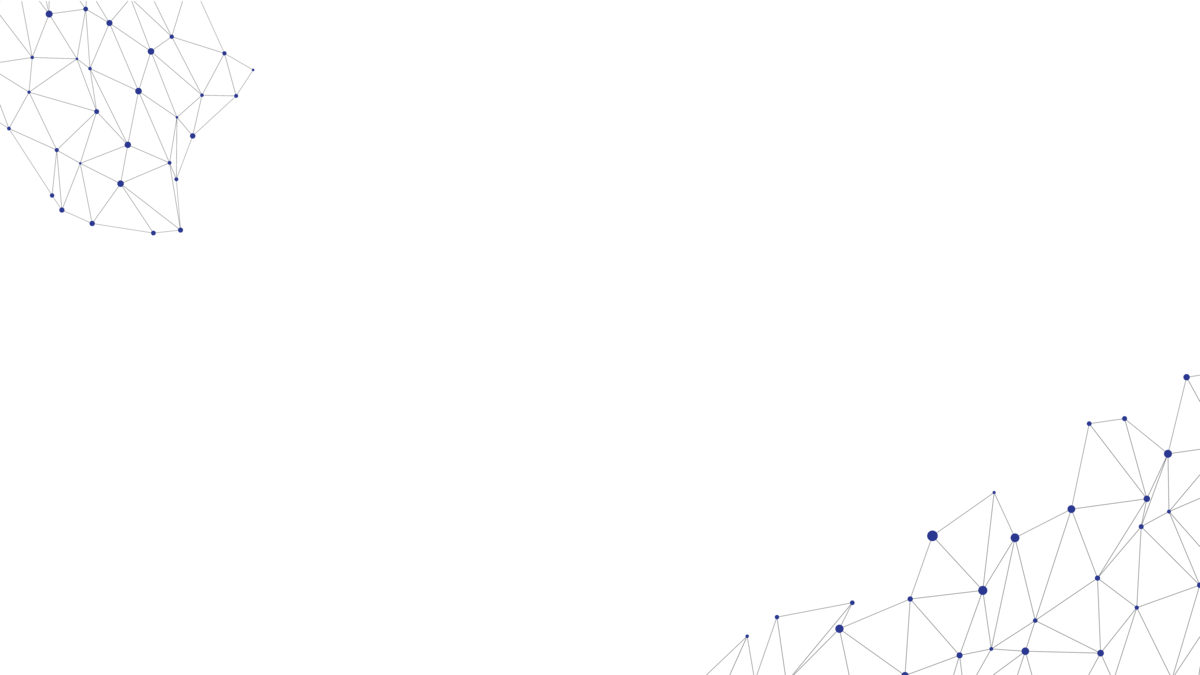
\includegraphics[width=\paperwidth]{Background 6.png}
}

% Title
\newcommand{\myTitle}
{
    Best customized Beamer Themes
}

% Subtitle
\newcommand{\mySubTitle}
{
    Beautiful title slides: Model 6
}

% Author
\newcommand{\myAuthor}   
{
    LaTeX-beamer.com
}

% Affiliation
\newcommand{\myAffiliate}
{
  Affiliation here
}

% Presentation Date
\newcommand{\myDate}   
{
    \today
}

% Logo
\newcommand{\myLogo}   
{
    \includegraphics[width=1cm]{Logo.png}
}
%%%%%%%%%%%%%%%%%%%%%%%%%%%%%%%%%%%%


%%%%%%%%%% Title slide code %%%%%%%%%%%
\begin{tikzpicture}[remember picture,overlay]

% Background color

\fill[white] (current page.south west) rectangle (current page.north east);
% Background image
\node[above right,inner sep=0pt] at (current page.south west)
    {
        \myBackround
    };
    
% Title & Subtitle
\node
[
    above=0.5cm,
    align=center,
    draw=black!50,
    % rounded corners,
    double,
    double distance=0.1cm,
    double=blue!10,
    fill=yellow!10,
    inner xsep=15pt,
    inner ysep=10pt, 
    minimum width=0.7\textwidth,
    text width=0.6\textwidth
] (title) at (current page.center)
{
    \LARGE \myTitle  \\[5pt]
    \small \mySubTitle
};

% Author 
\node[ below=0.5cm] (author) at (title.south){\myAuthor};

% Author 
\node[ below=0.25cm ](affiliate) at (author.south){\small \myAffiliate};

% Date
\node[below=0.25] (date) at (affiliate.south){\large \myDate};

% Logo
\node
[
    below =0.25cm
] at (date.south)
{
    %\myLogo
};

\end{tikzpicture}
    
\end{frame}

\section[Intro]{Objectives of this work}
\begin{frame}[t]{Setting: balance laws}
%	\MyLogoa
	
	\vspace{0.5cm}
	
	We want to solve numerically  hyperbolic systems of balance laws
	
	\begin{equation}
		\partial_tU+ \partial_x F(U)=  S(U)\partial_xH \nonumber
	\end{equation}
	
	\vspace{1.cm}
	
	Typical examples  that we will use here
	
	
	\begin{itemize}
		\item Burger's equations 
		\vspace{0.2cm}
		\item Shallow water equations with topography
		%\only<2->{\item{\bf Shallow water equations with topography/friction/Coriolis/etc}}
	\end{itemize}
	
	%\vspace{0.5cm}
%	
%	% \flushright{\underline{We  consider both 1D and Multi-D problems}}
%	%\only<1>{\color{white}{\\[5pt] But for simplicity the discussion is done for the 1D case}}
%	%\only<3>{\\[5pt]But for simplicity the discussion is done for the 1D case}
\end{frame}


\end{document}